% $Id: ESMF_superoverview.tex,v 1.2 2003/10/23 15:23:11 cdeluca Exp $
%
% Earth System Modeling Framework
% Copyright 2002-2003, University Corporation for Atmospheric Research, 
% Massachusetts Institute of Technology, Geophysical Fluid Dynamics 
% Laboratory, University of Michigan, National Centers for Environmental 
% Prediction, Los Alamos National Laboratory, Argonne National Laboratory, 
% NASA Goddard Space Flight Center.
% Licensed under the GPL.

%\section{Overview of Superstructure}

Component, State, and Transform objects are part of the Superstructure 
layer of the Earth System Modeling Framework (ESMF).  They encapsulate
computational models and the exchange of data between them.
They are designed to meet the requirements as specified in the
\htmladdnormallink{ESMF Requirements Document}{http://www.esmf.ucar.edu/esmf_docs/ESMF_reqdoc}.

A {\bf Component} 
is the highest level object in the ESMF object
hierarchy.  Components consist of user supplied code
which follows certain conventions defined by the ESMF framework. 
Components must provide a set of subroutines which match ESMF
defined interfaces. They must encapsulate
all their input and output data in an ESMF {\tt State} object.  They
must able to interpret an ESMF {\tt Time} object in order
to execute the requested number of model timesteps or time interval
before exchanging data with other Components.

Components are identified as being one or more of the
following subtypes: {\bf Application}, {\bf Gridded}, and {\bf Coupler}.  
An Application Component is the top level component which
contains other Components that cooperate in a computation. 
A Gridded Component
does the actual model computation.  A Coupler Component executes or
arranges the execution of the necessary data transformations between one
or more Gridded Components.


A {\bf State} 
encapsulates the data and sufficient description information
to allow the data computed by one Gridded Component to be
used as input to other Gridded Components.  A Gridded Component has
two states, an {\bf Import State} and an {\bf Export State}.
The Import State encapsulates all data needed as input to the
next timestep run of the Component.  The Export State encapsulates 
all data produced by the Component which is required by another
Component as input.  Data inside states are encapsulated by one 
or more of the following ESMF Objects: Bundles, Fields, or Arrays.
Components must exchange information with other Components
only by passing data through State objects.

A Coupler Component takes a list of State objects consisting of
both Export States and Import States.
The Coupler Component is responsible for transforming data 
so the appropriate Import States can be provided the corresponding
Component or Components.
The framework supplies
methods to do basic transformations which may include regridding,
interpolation, unit conversions, accumulations, averaging,
transformations which conserve specific values.


A {\bf Transform} object encapsulates a user-supplied function
containing the processing operations for coupling to be 
performed on a {\tt State} object.  For Components where it is not
feasible to return to the calling routine each time Coupling is
required, the Transform method can be called from within the
Component to perform the proper data transformations.

\newpage
\subsection{Object Model}

The following is a simplified UML diagram showing the relationships among
ESMF superstructure classes.  See Appendix A, {\it A Brief 
Introduction to UML},
for a translation table that lists the symbols in the diagram and their 
meaning.

\begin{center}
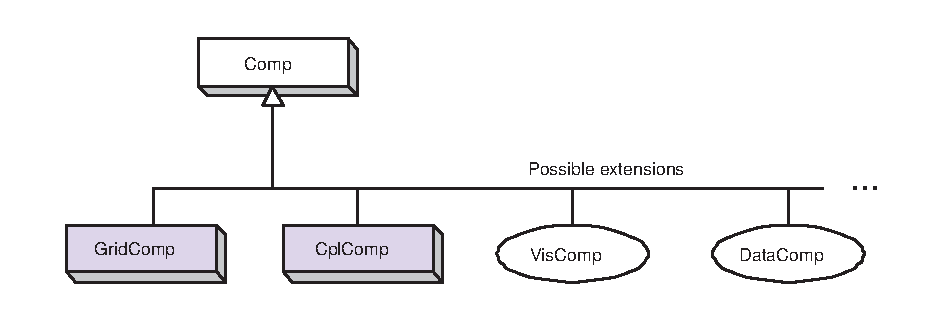
\includegraphics{Comp_obj.eps}   
\end{center}

